\chapter{Theory}\label{theory}
This chapter takes a closer look at the theory and technology applied in this thesis.

\section{Camera Calibration in OpenCV}
This section describes the theory behind the calibration process in OpenCV 4.3.0, which is the latest version at the time of writing this thesis.

\subsection{The pinhole camera model}
The functions OpenCV provides to calibrate the camera use the so-called pinhole camera model \cite{cv_calib}.
This model describes, how a 3D-point specified in world-coordinates ($P_w$) is transformed to a 3D-point in camera-coordinates ($P_c$) and then further projected onto the image plane ($p$). After this step, the point is described as a 2D-point in pixel coordinates.  Figure \ref{theory:pin} illustrates this setup.
\begin{figure}[ht]
	\centering
	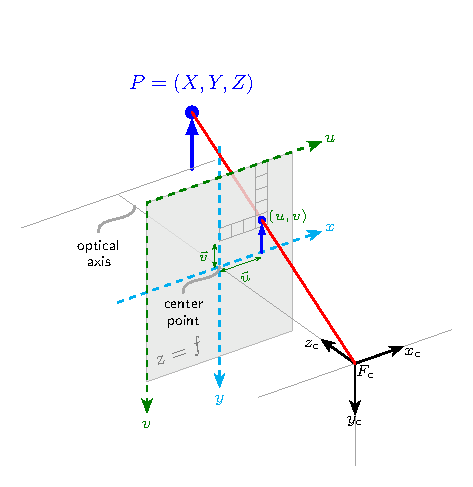
\includegraphics[width=0.9\textwidth]{2-theory/camera/camera.pdf}
	\caption{Pinhole-model (not up to date).\label{theory:pin}}
\end{figure} 

The transition from the world-coordinates to the camera-coordiantes can be described as 
\begin{align*}
\underbrace{\begin{pmatrix}
X_c\\
Y_c\\
Z_c\\
\end{pmatrix}}_{P_c}=
\underbrace{\begin{pmatrix}
r_{11}&r_{12}&r_{13}\\
r_{21}&r_{22}&r_{23}\\
r_{31}&r_{32}&r_{33}
\end{pmatrix}}_{R}
\underbrace{\begin{pmatrix}
X_w\\
Y_w\\
Z_w\\
\end{pmatrix}}_{P_w}+
\underbrace{\begin{pmatrix}
t_x\\
t_y\\
t_z\\
\end{pmatrix}}_{t}.
\end{align*}
The vector $P_w$ is first rotated by $R$ and the translated by $t$. This can be written in one single matrix:
\begin{align}
\begin{pmatrix}
X_c\\
Y_c\\
Z_c
\end{pmatrix}=
\begin{pmatrix}
r_{11}&r_{12}&r_{13}&t_x\\
r_{21}&r_{22}&r_{23}&t_y\\
r_{31}&r_{32}&r_{33}&t_z
\end{pmatrix}
\begin{pmatrix}
X_w\\
Y_w\\
Z_w\\
1
\end{pmatrix}\quad\Leftrightarrow\quad
P_c=
\begin{pmatrix}
R&|&t
\end{pmatrix}
\begin{pmatrix}
P_w\\
1
\end{pmatrix}\label{theory:world-camera}.
\end{align}

As a result of the theorem of intersecting lines, the projection from $P_c$ to $p$ is described as
\begin{align*}
\underbrace{\begin{pmatrix}
u\\
v
\end{pmatrix}}_{p}=
\begin{pmatrix}
f_x\cdot X_c/Z_c\\
f_y\cdot y_c/Z_c\\
\end{pmatrix}+
\begin{pmatrix}
c_x\\
c_y
\end{pmatrix}.
\end{align*}
where $f_x$ and $f_y$ are the focal length $f$ (in world units) normalized by their respective pixel size (in world units). Thus $f_x$ and $f_y$ are the same, if the pixels are quadratic.

By adding the principal point $\begin{pmatrix}c_x&c_y\end{pmatrix}^T$, which is usually close to the image center, it is taken into account, that pixel-coordinates are specified with respect to the upper left corner of the image plane. .
It is now simpler to write this in homogeneous coordinates:
\begin{align}
\begin{pmatrix}
u\\
v\\
1
\end{pmatrix}\sim s
\begin{pmatrix}
u\\
v\\
1
\end{pmatrix}=
\underbrace{\begin{pmatrix}
f_x&0&c_x\\
0&f_y&c_y\\
0&0&1
\end{pmatrix}}_{K}
\begin{pmatrix}
X_c\\
Y_c\\
Z_c
\end{pmatrix}\quad \Leftrightarrow \quad s
\begin{pmatrix}
p\\
1
\end{pmatrix}=
K\cdot P_c
\label{theory:camera-pixel},
\end{align}
where $s$ is an arbitrary scaling factor and $K$ is called the camera matrix.
The overall transition from world- to pixel-coordinates is the result of combining \ref{theory:world-camera} and \ref{theory:camera-pixel}:
\begin{align}
s
\begin{pmatrix}
u\\
v\\
1
\end{pmatrix}=
\begin{pmatrix}
f_x&0&c_x\\
0&f_y&c_y\\
0&0&1
\end{pmatrix}
\begin{pmatrix}
r_{11}&r_{12}&r_{13}&t_x\\
r_{21}&r_{22}&r_{23}&t_y\\
r_{31}&r_{32}&r_{33}&t_z
\end{pmatrix}
\begin{pmatrix}
X_w\\
Y_w\\
Z_w\\
1
\end{pmatrix}\quad \Leftrightarrow \quad s
\begin{pmatrix}
p\\
1
\end{pmatrix}=
K
\begin{pmatrix}
R&|&t
\end{pmatrix}
\begin{pmatrix}
P_w\\
1
\end{pmatrix}\label{theory:world-pixel}
\end{align}
The rotation and translation in $\begin{pmatrix}R&|&t\end{pmatrix}$ are called the extrinsic parameters. The camera matrix $K$ contains analogously the linear intrinsic parameters.

\subsection{The distortion model in OpenCV}
Non linear distortions, which appear before the projection in \ref{theory:camera-pixel} should be considered too. OpenCV implements the following model:
\begin{align}
\begin{pmatrix}
x''\\
y''
\end{pmatrix}=
\begin{pmatrix}
x'\frac{1+k_1 r^2+k_2 r^4+k_3 r^6}{1+k_4 r^2+k_5r^4+k_6r^6}+2p_1 x' y'+p_2(r^2+2x'^2)+s_1 r^2+s_2 r^4\\
y'\frac{1+k_1 r^2+k_2 r^4+k_3 r^6}{1+k_4 r^2+k_5r^4+k_6r^6}+2p_2x'y'+p_1(r^2+2y'^2)+s_3 r^2+s_4 r^4
\end{pmatrix}\label{theory:dist}
\end{align}
where $x'$ ad $y'$ are coordinates, described in camera-coordinates, normalized with $Z_c$
\begin{align*}
\begin{pmatrix}
x'\\
y'
\end{pmatrix}=
\begin{pmatrix}
X_c/Z_c\\
Y_c/Z_c
\end{pmatrix}
\end{align*}from
and r is the radius as taken with respect to the principal point $\begin{pmatrix}c_x&c_y\end{pmatrix}^T$
\begin{align*}
r^2 = x'^2 + y'^2.
\end{align*}
\cite{cv_calib}

In summary, a point in normalized camera-coordinates $\begin{pmatrix}x'&y'\end{pmatrix}^T$ is distorted as modeled in \ref{theory:dist}, which leads to the point $\begin{pmatrix}x''&y''\end{pmatrix}^T$. To get the distorted pixel-coordinates (subscript $d$), the projection has to be applied
\begin{align*}
\begin{pmatrix}
u_d\\
v_d\\
\end{pmatrix}=
\begin{pmatrix}
x''f_x+c_x\\
y''f_y+c_y
\end{pmatrix}\quad\Leftrightarrow\quad
\begin{pmatrix}
u_d\\
v_d\\
1
\end{pmatrix}=K
\begin{pmatrix}
x''\\
y''\\
1
\end{pmatrix},
\end{align*}
which completes the model so far. Keep in mind, that when correcting the distortion, equation \ref{theory:dist} has to be inverted.

By taking closer look at the coefficients in \ref{theory:dist}, one can see, that this model is a combination of different distortion models. The parameters $k_1$ to $k_6$ cause a distortion which is symmetric with respect to the principal point in the image plane. This so called radial distortion is caused by the lens, and usually dominates (paper von weng) 




